\documentclass[12pt, a4paper]{article}
% \usepackage[utf8]{inputenc}
\setlength{\parindent}{0pt}
\usepackage[dvips]{geometry}
% \usepackage[free-standing-units=true]{siunitx}
\usepackage{siunitx} % package for the units
\usepackage{graphicx} % package to manage images
\graphicspath{{./images/}}
\usepackage{amssymb}
\usepackage{subfig}
\geometry{a4paper,left=2cm,right=2cm, top=2cm, bottom=2cm}
\usepackage[version=4]{mhchem} % package for chemical equations
\usepackage{multirow} % merged rows in tables
\usepackage[style=numeric]{biblatex}

\addbibresource{refs.bib}

\begin{document}

% \begin{titlepage}
\includegraphics[width=0.3\textwidth]{images/kswe_logo.png}
\begin{center}
\vspace{5.5cm}
\Huge
\textbf{MATURAARBEIT}
\vspace{1cm}\\
\begin{LARGE}
A Quantitative Analysis of Homemade Sodium-Ion Batteries.\\
\end{LARGE}
\vspace{3.5cm}
\small
\textbf{supervised by}
\vspace{0.2cm}\\
Stefan Ibold
\vspace{1cm}\\
\textbf{submitted to}
\vspace{0.2cm}\\
Kantonsschule Wettingen\\
Klosterstrasse 11\\
5430 Wettingen
\vspace{1cm}\\
\textbf{submitted on}
\vspace{0.2cm}\\
the 7th of Nov 2022
\vspace{1cm}\\
\textbf{submitted by}
\vspace{0.2cm}\\
Adam Hoffman
\end{center}
\end{titlepage}

\begin{titlepage}
\begin{center}
\textbf{International Baccalaureate Diploma Program}
\vspace{10cm}\\
\Huge
\textbf{Extended Essay Chemistry}
\vspace{0.5cm}\\
\LARGE
A Quantitative Analysis of Homemade Sodium-Ion Batteries.
\vspace{8.5cm}\\
\small
\textbf{Words: 3923}\\
\textbf{Pages: 21}
\vfill
\date{\today}
\end{center}
\end{titlepage}

\newpage

\tableofcontents

\newpage
\section{Abstract}
Electricity is based on the movement of charged matter. Through the work done upon a moving charge in an electric field, a potential emerges. Through the formation of a circuit, the potential causes a current to flow and consequently energy to be transmitted\cite{Kammer2019}.\\
Electric energy powers most of modern infrastructure and has become an essential pillar of almost every facet of modern life. With the only limitation being the need of electric outlets. However, with the development of the battery, mobile electronic devices have taken over the modern lifestyle and made the battery one of the most important components in the general field of electronics. Nonetheless, the current rechargeable, consumer battery market is dominated by lithium-ion technology, which comes with a variety of disadvantages, such as the environmental impacts of lithium, the danger of thermal runaway and the depletion of resources\cite{Peters2017, Peters2016, Wang2012}. This experiment investigates the construction process and the viability of a sequence of homemade sodium-ion batteries. The batteries are constructed using a graphite anode and a titanium-dioxide cathode separated by a layer of tape, with a 1 mol/L sodium-perchlorate aqueous solution acting as the electrolyte. In separate trials with varying cathode thickness, anode substance and battery form-factor, the battery voltage, discharge current, as well as multiple discharge curves are determined. The results are tabulated and compared with a state-of-the-art lithium battery, while taking into consideration the limitations of the experiment. The average capacities achieved are \SI{5.52e-3}{\mA\hour} and \SI{3.18e-3}{\mA\hour} with maximum power outputs of \SI{1.01e-3}{\W} and \SI{3.30e-4}{\W}. While this does not currently outperform any commonly available battery, the value of this experiment lies in the proof of concept: Detailing the construction of an easily built, cheap, and safe alternative to the common lithium-ion battery. With only minimal investment, the technology presented could prove a sustainable future for batteries.
\newpage
\section{Introduction}
\subsection{Real-World Relevance}
Charge is considered a fundamental property of matter. Even though multiple charged particles exist, in practice the electron is of greatest use in the field of electronics. Through the loss or gain of electrons, an electric charge is built-up and consequently, an electric field emerges. When placing a charge in an electric field, a force is applied to the charge. In consequence, when placing a travelling charge in an electric field, work is done upon the charge by the field\cite{Kammer2019}. Thus, a potential capable of producing a current arises, commonly called electricity. Over the past two decades, electricity has become essential in our day-to-day life. In the last 40 years alone, the net world wide yearly consumption of electricity has more than tripled, from \SI{7323}{\tera\W\hour} to \SI{23845}{\tera\W\hour}\cite{Alves2022}. Similarly, the access to electricity has increased from \SI{78.2}{\percent} to over \SI{90}{\percent} throughout the past 20 years alone\cite{WorldBank2020}. At this point, life without a large-scale electricity infrastructure would be inconceivable.

A battery is a device capable of storing electrical energy as chemical energy and releasing it in form of electricity\cite{Bates2012}. As the first effective storage medium for electricity, the battery is the foundation of modern portable electronics. Through the past 200 years, humanity has been perfecting the battery to supply evermore powerful devices with electricity\cite{Schumm2022}. Currently, nickel-metal-hybrid and lithium-ion technologies dominate the rechargeable-battery consumer market and are the second and third most used household batteries respectively\cite{Schumm2022}.\\
With the increase in sales of portable electronic devices, as shown in Fig. \ref{fig:smartphonesales}, as well as the increase in electric vehicle production and the recent surge towards renewable and eco-friendly energy engineering, the battery has become an essential foundation in many aspects of the modern lifestyle\cite{Laricchia2022,Tarascon2010,Relations2022}.
Particularly its use to counteract the inconsistent electricity production of renewable energy sources such as windfarms or solar panels, has given electrical energy storage a key role in the fight against global warming.

\begin{figure}[ht]
    \centering
    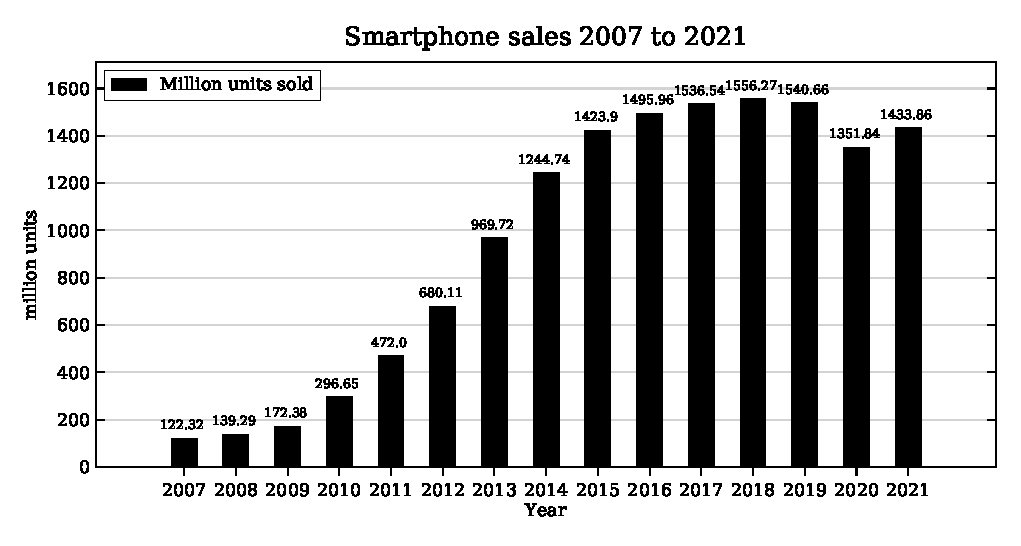
\includegraphics[width=\textwidth]{images/phonesales.eps}
    \caption{Number of smartphones sold to end users per annum from $2007$ to $2021$ in million units.}
    \label{fig:smartphonesales}
\end{figure}

\newpage

However, lithium-ion batteries are limited in multiple ways. Their construction promotes resource depletion and the release of poisonous substances into the environment \cite{Mrozik2021} - most notably, the use of rare metals such as cobalt, the estimated two million liters of water required for the mining of one metric ton of lithium, as well as the devastating impacts of toxic chemicals used for the extraction of lithium\cite{Katwala2018,Peters2017}. To prevent further pollution and help fight the global environmental crisis, more eco-friendly technologies are required. Sodium-ion batteries (SIBs) offer such a potential. Not only is sodium roughly 1000 times more naturally abundant than lithium, but its extraction also does not require harmful substances\cite{WikipediaAbun2022}. Furthermore, no rare metals are needed for the construction of sodium-ion batteries and their operation is less prone to thermal runaway\cite{Peters2016}. 

This investigation aims to assess the effectiveness and viability of homemade SIBs in the context of cost, safety, and environmental impact, while considering the production process as well as other state-of-the-art batteries.

\subsection{Investigation Context and Research Question}
The initial idea for the experiment is based on a sequence of videos published on YouTube\cite{Youtube2019}. They demonstrate the development of a solid-state sodium-ion battery constructed out of household materials over a period of multiple years. The core components include a graphite anode and a toothpaste cathode without an electrolyte and separator. However, these results were not reproducible. Furthermore, there was no research found to support these experiments. Most likely, the batteries seen in the videos are backed by years of experience and experimentation, which were non-replicable.

Thus, the scope of this investigation was adjusted to entail the construction of a sodium-ion battery and its evaluation in terms of viability and efficiency. Consequently, the following research question was chosen: To what extent are homemade sodium-ion batteries a viable and effective replacement for modern, state-of-the-art rechargeable batteries?.

Being restricted by the capabilities of a school laboratory, this experiment is unable to compete with cutting-edge research done around the world. However, since the core technology behind SIBs is comparatively simple, the focus was set on a more real-world relevant experiment. Based on instructions published by the University of Education in Freiburg, a simple sodium-ion accumulator is designed, constructed, and evaluated\cite{Klaus2022}. At its core, the battery consists of a titanium-dioxide layer applied to a fluorine-doped tin oxide (FTO) coated glass slide as a cathode, a graphite coated FTO glass slide as an anode and a sodium perchlorate solution as an electrolyte, based upon the instructions found online\cite{WikipediaFTO2022}.
FTO glass slides are chosen as current collectors to minimize the differences to a known, functional experiment and thus limit the sources of error. Further, titanium-dioxide and graphite are chosen, thanks to their ability to intercalate perchlorate ions and their use as both anodes and cathodes in previous works\cite{Guo2016}.
Due to substance limitations, the electrolyte was adapted, and de-ionized water is chosen, because of its use in aqueous sodium-ion batteries\cite{Che2017}. 
To evaluate the viability and efficiency, the battery's open circuit voltage, discharge curve and capacity are assessed and compared to a state-of-the-art lithium-ion battery by Panasonic\cite{Panasonic2018}. 
Furthermore, the process of construction, as well as the general state of knowledge concerning the field of sodium-ion batteries is taken into consideration.
\newpage
\section{Theory}
All the terms utilized throughout this paper attain their meaning from the field of electrochemistry, unless specified otherwise. Furthermore, \textit{cathode} refers to the negative pole during process and the \textit{anode} refers to the positive pole during discharge.

\subsection{Sodium-Ion Batteries}
At their core, all modern batteries are based on a redox reaction. Through the exchange of electrons accompanying a sequence of oxidation and reduction, a charge can be stored and released\cite{Beerenwinkel2012}.
This is commonly facilitated through two electrodes capable of intercalating ions, separated by a separator and electrically connected through a conductive electrolyte. In the field of sodium-ion batteries (SIBs), layered-metal-oxide and a polyanionic anode are commonly paired with a hard-carbon cathode and a liquid carbonate ester electrolyte\cite{Xiang2015,Che2017,Xie2020}.
Solid electrolytes exist but are less common\cite{Dai2021}. Through the intercalation of sodium-ions in the hard-carbon during the charging process, a charge and thus a potential is built up between the two electrodes, which can be harnessed as electrical energy during discharge. Most commonly, the sodium-ions are transferred from the anode to the cathode upon charge and returned upon discharge.
The experiment performed during this investigation slightly alters this process and only exchanges the sodium-ions between the cathode and the electrolyte. In the discharged state, the sodium-ions are bound to perchlorate in the electrolyte solution and only intercalate in the TiO2 cathode upon the application of a current to the cathode through the charging process, as explained by Wu Liming et al\cite{Wu2015} and as visible in equation \ref{eq:sodiumintercalation}. This reduction requires the addition of electrons. Concurrently, the perchlorate-ions are intercalated in the graphite anode, as seen in equation \ref{eq:perchlorateintercalation}. This oxidation releases electrons. The charging process can thus be represented by the following reactions taking place at the two electrodes concurrently.

\begin{align}\label{eq:sodiumintercalation}
    \ce{TiO2 + NaClO4 + e- &-> NaTiO2 + ClO4- \\\label{eq:perchlorateintercalation}
    C6 + NaClO4 &-> C6 ClO4 + Na+ +e-}
\end{align}

During discharge, the reversed reactions occur at the same electrodes to facilitate a reversed current flow through an external circuit, where electrons would be taken up by the anode and released by the cathode. Thus, a complete reaction of the battery constructed is shown in eq. \ref{eq:fullbatteryeq}, with the charging process being visible from left to right and the discharge from right to left.

\begin{equation}\label{eq:fullbatteryeq}
    \ce{C6 + NaClO4 + TiO2 <=> C6 ClO4 + NaTiO2}
\end{equation}

\begin{figure}[ht]
    \centering
    \includegraphics[width=\textwidth]{images/sodium_ion_battery_figure.png}
    \caption{A diagram depicting the basic layout of a sodium-ion battery.}
    \label{fig:sodiumbatterydiagram}
\end{figure}

\newpage

\subsection{Battery Evaluation}

To help compare and evaluate a battery, its capacity and power can be calculated. The capacity, also known as the charge, is based on total current flow, as visible in equation \ref{eq:capacityequation}:

\begin{equation}\label{eq:capacityequation}
    I = \frac{\Delta Q}{\Delta t} \Rightarrow \Delta Q = I \cdot \Delta t
\end{equation}
\begin{align*}
    Q &: \text{Capacity in coulombs [\unit{\C}]}\\
    I &: \text{Current in amperes [\unit{\A}]}\\
    t &: \text{time in seconds [\unit{\s}]}
\end{align*}

Similarly, the average power can be determined through the average current and average voltage, as seen in equation \ref{eq:powerequation}:

\begin{equation}\label{eq:powerequation}
    P = U \cdot I
\end{equation}
\begin{align*}
    P &: \text{Electric power in watt [\unit{\W}]}\\
    U &: \text{Voltage in [\unit{\V}]}
\end{align*}
\newpage
\section{Methods}
The experimentation process can be divided into three stages: 
\begin{enumerate}
    \item Electrode construction
    \item Battery assembly
    \item Evaluation process
\end{enumerate}

In total, seven individual variables are assessed, of which the cathode layer-thickness, anode carbon source and evaluation process, which includes the charge time and the discharge load, will be presented in more detail. The investigation of the titanium-dioxide powder used, the sodium-perchlorate concentration as well as the battery form factor will be briefly mentioned, however, they were evaluated as being less impactful on the battery effectiveness.

\subsection{Cathode Layer Thickness}
\subsubsection{Experiment Design}
The core substance comprising the cathode is titanium-dioxide, as it can effectively intercalate sodium-ions and is commonly used as both anodes and cathodes in sodium-ion batteries\cite{Guo2016}.
In essence, the cathode is made up of a FTO glass slide acting as the current collector, coated with a titanium-dioxide suspension, and left to sinter in a drying oven. Different thicknesses of titanium-dioxide layers are investigated, with the aim to create a conductive titanium-dioxide coating. The actual performance in a battery was not measurable during the experiment, as this part of the investigation was completed before an actual battery was constructed and acted as a precursor to the battery design process.

\subsubsection{Variables}
\begin{table}[h]
\renewcommand{\arraystretch}{1.3}
\caption{Iteration Parameters}
\label{table:parameterscathode}
\centering
\begin{tabular}{l|l|l||l}
\multicolumn{3}{c||}{\bfseries Parameter}&\bfseries Values\\
\hline
\hline
\multicolumn{2}{c|}{\multirow{2}{*}{Constant}}&The current collector&FTO slide\\
\cline{3-4}
\multicolumn{2}{c|}{}&The cathode substance&Titanium-dioxide\\
\hline\hline
\multirow{2}{*}{Varying}&Independent&The TiO$_2$ layer thickness&$\approx$\SI{1}{\mm}, $\approx$\SI{1.5}{\mm}, $\approx$\SI{2}{\mm}\\
\cline{2-4}
&Dependent&The conductivity of the TiO$_2$ layer&To be measured\\
\end{tabular}
\end{table}
            
\subsubsection{Process}
\begin{enumerate}
\item The FTO glass slides are cleaned using a general cleaning solution, followed by a glass specific cleaner.
\item A diluted nitric-acid solution is created by diluting \SI{1}{\ml} of a \SI{1}{\mol\per\L} nitric-acid solution with \SI{1000}{\ml} of de-ionized water. The dilution ratio is negligible, whereas a pH between 3-4 is critical.
\item Next, \SI{6}{\g} of Degussa titanium-dioxide powder is added to \SI{12}{\ml} of the diluted nitric-acid solution and crushed using a glass rod to ensure total suspension.
\item Subsequently, three FTO glass slides are prepared by taping off three of their sides with thin scotch tape. Approximately $3$ to \SI{4}{\mm} of each edge should be covered by tape.
\item Next, 1 droplet of the titanium-dioxide suspension is applied to the first slide with a single-use pipette. 2 droplets are applied to the second and 3 droplets to the third slide. The droplets are positioned on one of the taped-off sides between two strips of tape while touching the third.
\item The titanium-dioxide suspension is then spread over the entire surface of the FTO glass slide with a glass rod. As the rod is moved from side a to b it glides directly on top of the taped edges. Thus the thickness of the tape determines the pressure applied while spreading the suspension and therefore serves as a measure of layer thickness. It is recommended to swivel the glass rod right to left in the droplets prior to spreading the suspension, thus ensuring full coverage of the glass slide. The entire surface can be covered with a single motion, which results in a more even coating.
\item The coated slides are air-dried for \SI{10}{\minute}. The tape is removed and the slides are then placed in a drying oven to sinter at \SI{200}{\degreeCelsius} for another \SI{10}{\minute}.
\item Finally, the resistance between the FTO coating and the titanium-dioxide layer is measured with a multimeter. The first probe is placed directly upon the FTO coating on one of the open edges previously covered by tape, while the second is placed directly upon the titanium-dioxide layer.
\end{enumerate}
            
\begin{figure}[ht!]
\centering
\subfloat[]{\includegraphics[width=0.331\textwidth]{taped_cathode.jpg}}
\subfloat[]{\includegraphics[width=0.338\textwidth]{coated_cathode.jpg}}
\subfloat[]{\includegraphics[width=0.331\textwidth]{final_cathode.jpg}}
\caption{(a): An FTO slide prepared by taping off three of the four sides. (b): An FTO slide after the titanium-dioxide coating. (c): The final cathode after sintering.}
\label{fig:cathodeprocess}
\end{figure}

\newpage

\subsection{Anode Carbon Source}
\subsubsection{Experimental Design} 
The anode is comprised of graphite, even though it is known that sodium-ions do not intercalate well in graphite and hard carbon should be used instead\cite{Xie2020}. However, since this experiment intercalates perchlorate ions in the graphite anode, this limitation can be disregarded. 
Three different sources of carbon are compared in terms of their use in a battery stack: An IKEA tea light candle, a Faber Castell pure graphite pencil and a laboratory grade graphite anode\cite{Ikea2022, Castell2022}.
The effectiveness is measured by determining the battery charge voltage, discharge voltage and peak discharge current over a \SI{1e3}{\ohm} resistance.

\subsubsection{Variables}
\begin{table}[h]
\renewcommand{\arraystretch}{1.3}
\caption{Iteration Parameters}
\label{table:parametersanode}
\centering
\begin{tabular}{l|l|l||l}
\multicolumn{3}{c||}{\bfseries Parameter}&\bfseries Values\\
\hline
\hline
\multicolumn{2}{c|}{\multirow{2}{*}{Constant}}&The current collector&FTO slide\\
\cline{3-4}
\multicolumn{2}{c|}{}&The anode substance&Carbon\\
\hline\hline
\multirow{2}{*}{Varying}&Independent&The carbon source&Graphite, soot, pencil\\
\cline{2-4}
&\multirow{2}{*}{Dependent}&The charged voltage in a battery&To be measured\\
\cline{3-4}
&&The discharge current in a battery&To be measured\\
\end{tabular}
\end{table}
    
\begin{figure}[ht!]
\centering
\subfloat{\includegraphics[width=0.427\textwidth]{soot_anode.jpg}}
\subfloat{\includegraphics[width=0.573\textwidth]{graphite_anode.jpg}}
\caption{(a): FTO slide covered in candle soot. (b): FTO slide coated with a pure graphite pencil.}
\label{fig:anodefig}
\end{figure}
    
\subsubsection{Process}

\begin{enumerate}
\item First, the FTO glass slides are cleaned using a general cleaning solution, followed by a glass specific cleaner.
\item Next, the tea light candle used is lit beforehand to ensure a steady and even flame during the experiment.
\item Additionally, the laboratory grade graphite electrode is roughed up using 80 grit sandpaper, to remove any substances obstructing the surface.
\item Subsequently, the two FTO glass slides are prepared by taping off a single side on the first slide and three sides on the second slide. Approximately \SI{3}{\mm} of each edge are covered with tape.
\item The FTO glass slide with three taped-off sides is covered in soot, by passing it over the pre-lit candle multiple times in quick succession. The slide is held a few millimetres above the wick and is continuously passed over the flame until an even coating of soot is achieved.
\item The FTO glass slide with a single taped-off side is covered by a layer of graphite using the pure graphite pencil. It is continuously painted until a homogeneous gray color is achieved and no obvious stroke marks are visible.
\item Finally, the tape is removed, and the cathodes are tested in a battery setting. The battery layout is described below.
\end{enumerate}

\begin{figure}[ht!]
\centering
\includegraphics[width=\textwidth]{final_anode.jpg}
\caption{The final anode used, created by utilizing the graphite pencil.}
\label{fig:finalanode}
\end{figure}

\newpage

\subsection{Battery Evaluation Process}
\subsubsection{Experiment Design}
Throughout the construction process, the effectiveness of the individual components are assessed by different means. However, the final battery produced is evaluated according to three different discharge curves measured on two different batteries.
The curves are determined by connecting the charged battery to a constant load and measuring the current and the voltage over a period of time with a multimeter. 
A detailed circuit diagram can be seen in Fig. \ref{fig:circuitfig}. 
Three different discharge curves are measured. Two after a \SI{10}{\minute} charge with a \SI{1e3}{\ohm} resistor and a \SI{1e2}{\ohm} resistor respectively and the third after a \SI{20}{\minute} charge with a \SI{1e3}{\ohm} resistor. A recording period of 10 minutes is chosen, since the obtained values quickly fall below a significant value and a longer measuring period would be redundant.

\subsubsection{Variables}
\begin{table}[h]
\renewcommand{\arraystretch}{1.3}
\caption{Iteration Parameters}
\label{table:parametersbatteryevaluation}
\centering
\begin{tabular}{l|l|l||l}
\multicolumn{3}{c||}{\bfseries Parameter}&\bfseries Values\\
\hline
\hline
\multicolumn{2}{c|}{\multirow{3}{*}{Constant}}&The batteries utilized&Constructed as described above\\
\cline{3-4}
\multicolumn{2}{c|}{}&The charging voltage&\SI{4.6}{\volt}\\
\cline{3-4}
\multicolumn{2}{c|}{}&The discharge temperature&Room temperature (\SI{20}{\degreeCelsius})\\
\hline\hline
\multirow{2}{*}{Varying}&\multirow{2}{*}{Independent}&The discharge load&\SI{1e2}{\ohm} and \SI{1e3}{\ohm}\\
\cline{3-4}
&&The charge time&\SI{10}{\minute} and \SI{20}{\minute}\\
\cline{2-4}
&\multirow{2}{*}{Dependent}&The discharge current over time&To be measured\\
\cline{3-4}
&&The discharge voltage over time&To be measured\\
\end{tabular}
\end{table}

\begin{figure}[ht!]
\centering
\includegraphics[width=\textwidth]{circuit.png}
\caption{The circuit used to measure the discharge curves.}
\label{fig:circuitfig}
\end{figure}

\newpage
    
\subsubsection{Process}
\begin{enumerate}
\item The battery is constructed and charged for \SI{10}{\minute} at a constant voltage of \SI{4.6}{\volt}.
\item The battery is then connected to the above described measuring circuit with a \SI{1e3}{\ohm} resistor and left to discharge for \SI{10}{\minute}.
\item The battery is recharged for \SI{10}{\minute} at a constant voltage of \SI{4.6}{\volt}.
\item It is again connected to the measuring circuit and discharged over a \SI{1e2}{\ohm} resistor for \SI{10}{\minute}.
\item The battery is recharged for \SI{20}{\minute} at a constant voltage of \SI{4.6}{\volt}.
\item The discharge curve is measured with a \SI{1e3}{\ohm} resistor for \SI{10}{\minute}.
\item This process is repeated for the second battery
\end{enumerate}

\subsection{Other Experiments}
The titanium-dioxide powder used was evaluated, since the origin of the powder initially utilized was unknown and thus considered a potential limitation. However, it was concluded, that the powder used initially, labelled with \textit{Degussa}, is the most suited for the task.

\begin{figure}[ht!]
\centering
\includegraphics[width=\textwidth]{different_titanium_dioxide_powder.png}
\caption{The different titanium-dioxide powders investigated.}
\label{fig:otherexp}
\end{figure}

The sodium-perchlorate concentration was investigated by creating three different batteries as per the method described above. They were filled with a \SI{0.2}{\mol\per\L}, a \SI{0.5}{\mol\per\L} and a \SI{1}{\mol\per\L} sodium-perchlorate, de-ionized water solution respectively, which acts as the electrolyte. It was concluded that \SI{1}{\mol\per\L} is the most effective electrolyte concentration. The evaluation of this experiment was out of scope of this investigation.

Two different battery form factors were evaluated. However, only a stack-based approach, with the electrodes being placed on top of one another and the electrolyte together with the tape separator in between, managed to function as a battery. The initial layout, as described in the reference experiment, suffered from various limitations\cite{Klaus2022}.

\begin{figure}[ht!]
\centering
\includegraphics[width=\textwidth]{final_setup.jpg}
\caption{The stack-based battery form factor.}
\label{fig:finalsetup}
\end{figure}
\newpage
\section{Safety Guidelines}
When working with electric circuits, the danger of getting electrocuted is always present, particularly when working with open circuits and self-made batteries, since the chance of touching a live component is increased. However, since the power of the batteries constructed is insignificant, this danger is limited when working with the battery alone. During the charging process on the other hand, special attention must be paid, since the battery is connected to a constant \SI{4.6}{\V} which can be lethal at high enough amperage. This is again limited by the modern security equipment present in every laboratory, with fuses protecting the connections from drawing too much current upon a touch.\\
Furthermore, some of the substances used require special attention. The \SI{1}{\mol\per\L} nitric acid utilized to create titanium-dioxide suspensions must be exclusively handled with gloves and disposed of correctly. Moreover, the titanium-dioxide powder in its raw form is labelled as a potential occupational carcinogen when inhaled. When handling the powder in its pure form, a fume hood prevents contact with the respiratory system \cite{Prevention2019}. However, since the powder was mostly handled in a suspended form, these dangers only apply during the suspension creation process.\\
Finally, caution is required when handling sodium-perchlorate since it is a reactive chemical and an explosion hazard when dried-out. Thus, the anhydrous sodium-perchlorate, as well as the electrolyte solution used were always kept in firmly closed, air-tight containers to prevent drying-out.

\newpage
\section{Results}
\begin{figure}[ht!]
\centering
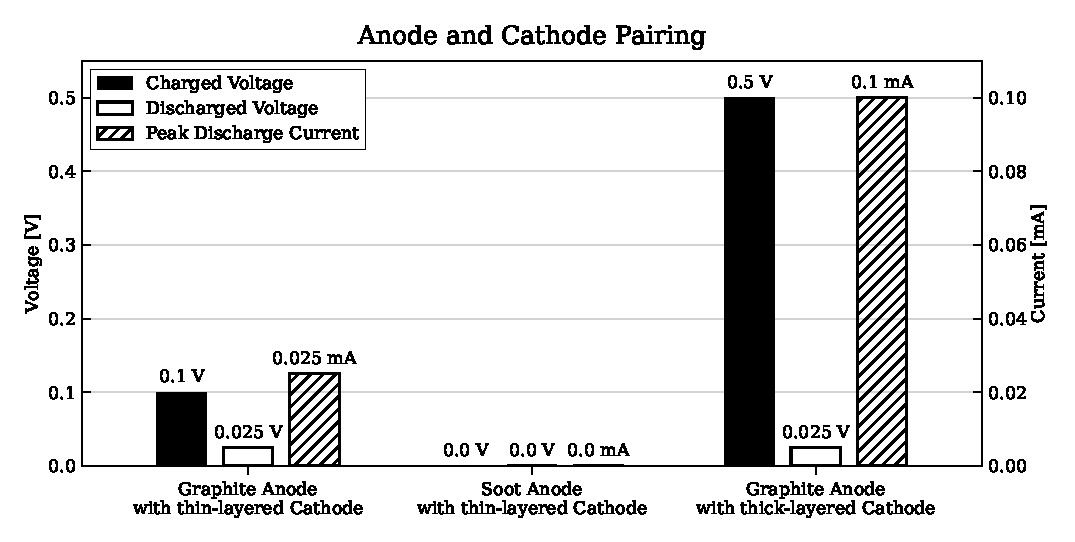
\includegraphics[width=\textwidth]{images/batteryfig.eps}
\caption{The charged and discharged voltage, as well as the peak discharge current of different anode and cathode pairings.}
\label{fig:anodecathodepairing}
\end{figure}

\begin{figure}[ht!]
\centering
\includegraphics[width=0.9\textwidth]{broken_cathode}
\caption{The cathode permanently damaged by the electrolysis of water.}
\label{fig:brokencathode}
\end{figure}

\begin{figure}[ht!]
\centering
\subfloat[]{\includegraphics[width=0.256\textwidth]{broken_soot_anode}}
\subfloat[]{\includegraphics[width=0.388\textwidth]{degraded_cathode}}
\subfloat[]{\includegraphics[width=0.353\textwidth]{cracked_cathode}}
\caption{(a): The soot anode during use. (b): A degraded cathode. (c): A too thick, cracked cathode.}
\label{fig:degradedelectrodes}
\end{figure}

\begin{figure}[ht!]
\centering
\subfloat[]{\includegraphics[width=0.443\textwidth]{charged_thick_cathode}}
\subfloat[]{\includegraphics[width=0.557\textwidth]{charged_thin_cathode}}
\caption{(a): A charged, thick-layered cathode. (b): A charged, thin-layered cathode.}
\label{fig:chargedchathodes}
\end{figure}

\newpage
    
As shown in Fig. \ref{fig:anodecathodepairing}, a thick titanium-dioxide layer effectively outperforms a thinner layer both in terms of the charged to discharged voltage difference and the peak discharge current.
The thin-layered cathode achieves a charged to discharged difference of $\Delta_{\text{thin}} = \SI{0.1}{\V} - \SI{0.025}{\V} = \SI{0.075}{\V}$ compared to the $\Delta_{\text{thick}} = \SI{0.5}{\V} - \SI{0.025}{\V} = \SI{0.475}{\V}$ charged to discharged delta presented by the thick-layered cathode.

In terms of peak discharge current, the thick-layered cathode outperforms the thin-layered cathode by a factor of four. However, as visible in Fig. \ref{fig:degradedelectrodes} (c) a thicker layer of titanium-dioxide is prone to cracks and disconnect from the FTO current collector. This leads to faster cathode degradation, shown in Fig. \ref{fig:degradedelectrodes} (b). After just a few discharge cycles, a large part of the titanium-dioxide coating has fallen off, and the cathode is burnt. 
However, a thinner titanium-dioxide layer offers less sodium-ion storage. This can be seen through the difference in color intensity between a charged, thin titanium-dioxide coating and a charged, thick coating in Fig. \ref{fig:chargedchathodes}. The thick-layered cathode (a) is visibly more blue than the thin-layered cathode (b), which indicates a higher quantity  of intercalated sodium-ions.
Furthermore, as visible in Figs. \ref{fig:anodecathodepairing} and \ref{fig:degradedelectrodes} (a), soot as an anode substance is not compatible with a water-based electrolyte, as it suspends in the aqueous solution and detaches from the FTO glass slide.

\newpage

\begin{figure}[ht!]
\centering
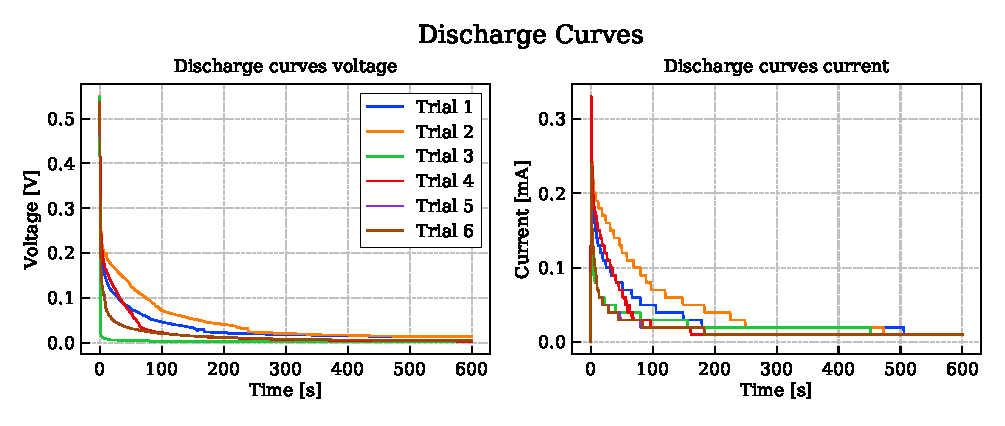
\includegraphics[width=\textwidth]{images/dischargefig.eps}
\caption{The voltage and current discharge curves of two different batteries over two different loads with varying charge times.}
\label{fig:dischargecurves}
\end{figure}

\begin{table}[ht!]
\centering
\begin{tabular}{c||c|c}
\bfseries Trial & \bfseries Charge time & \bfseries Resistance \\
\hline\hline
Trial 1 & \multirow{2}{*}{\SI{10}{\minute}} &\SI{1e3}{\ohm} \\
\cline{1-1}\cline{3-3}
Trial 2 &&\SI{1e2}{\ohm} \\
\hline
Trial 3 & \SI{20}{\minute} &\SI{1e3}{\ohm} \\
\hline
Trial 4 & \multirow{2}{*}{\SI{10}{\minute}} &\SI{1e3}{\ohm} \\
\cline{1-1}\cline{3-3}
Trial 5 &&\SI{1e2}{\ohm} \\
\hline
Trial 6 & \SI{20}{\minute} &\SI{1e3}{\ohm} \\
\hline
\end{tabular}
\caption{Trial descriptions.}
\label{tab:trialdescriptions}
\end{table}

The discharge curves obtained do not resemble those produced by commercially available batteries, since no rated voltage is held over a longer period \cite{Panasonic2018}. Instead, both the voltage and current discharge curves decline rapidly. 
As can be expected through the relationship between current, voltage and resistance: $\mathrm{U}=\mathrm{R} \cdot \mathrm{I}$ and as visible through the grey and green curves in Fig. \ref{fig:dischargecurves}, a lower load resistance of \SI{1e2}{\ohm} compared to \SI{1e3}{\ohm} results in a lower voltage curve overall.
Counterintuitively, the corresponding current curves similarly dropped overall, instead of increasing.
Furthermore, a longer charging period seems to impact battery 1, but not battery 2, as displayed by the generally higher orange curve compared to the more average brown curve in Fig. \ref{fig:dischargecurves}.

\newpage

\subsection{Data Analysis}
The capacity of the batteries can be determined by integrating the current discharge curves and calculating the area under the curve, as described in equation \ref{eq:capacityequation} and demonstrated in equation \ref{eq:capacityexample}. The integral was numerically approximated using the midpoint rule and a discretization time-step $\Delta t = t_i - t_{i-1} = \SI{1}{\second}$\cite{Kammer2019}.

\begin{align}\label{eq:capacityexample}
    Q &= \int_0^T I \cdot t \cdot d t \approx \sum_{i=1}^{T} \frac{I_i + I_{i-1}}{2} \cdot (t_{i}-t_{i-1}) \Rightarrow Q = \SI{1.92e-2}{\coulomb} \quad \text{duration } T = \SI{600}{\second}\\
    Q &= \SI{5.33e-3}{\mA\hour}
\end{align}


Additionally , the average power output can be calculated, by multiplying the average current by the average voltage. As mentioned in equation \ref{eq:powerequation} and demonstrated in equation \ref{eq:powerexample}.

\begin{align}\label{eq:powerexample}
    I_\text{average} &= \frac{1}{n}\sum_{i=1}^{n} I_i \Rightarrow I_\text{average} = \SI{3.19e-5}{\ampere} \quad \text{duration } n = \SI{600}{\second}\\
    U_\text{average} &= \frac{1}{n}\sum_{i=1}^{n} U_i \Rightarrow U_\text{average} = \SI{3.14e-3}{\volt} \quad \text{duration } n = \SI{600}{\second}\\
    P_\text{average} &= I_{\text{average}} \cdot  U_\text{average} = \SI{3.2e-5}{\ampere} \cdot \SI{3.14e-3}{\volt} = \SI{1.00e-3}{\watt}\\
\end{align}

All calculations were done in Microsoft Excel and can be verified online\cite{Hoffman2022}.

\begin{table*}[!ht]
\renewcommand{\arraystretch}{1.3}
\centering
\begin{tabular}{c |c |c||c|c}
\bfseries Trial & $T_\text{charge}$ [\unit{\min}] & Resistance [\unit{\ohm}] & $Q$ [\unit{\mA\hour}] & $P_\text{average}$ [\unit{\W}]\\
\hline\hline
\multirow{3}{*}{Battery 1}&\multirow{2}{*}{$10$}&\num{1e3}&\num{5.33e-3}&\num{1.00e-3}\\
\cline{3-5}
& &\num{1e2}&\num{3.89e-3}&\num{7.29e-5}\\
\cline{2-5}
&$20$&\num{1e3}&\num{7.33e-3}&\num{1.96e-3}\\\hline\hline
\multicolumn{3}{c||}{\bfseries Average}&\num{5.52e-3}&\num{1.01e-3}\\\hline\hline
\multirow{3}{*}{Battery 2}&\multirow{2}{*}{$10$}&\num{1e3}&\num{3.83e-3}&\num{4.75e-4}\\
\cline{3-5}
& &\num{1e2}&\num{2.85e-3}&\num{2.58e-4}\\
\cline{2-5}
&$20$&\num{1e3}&\num{2.85e-3}&\num{2.57e-4}\\\hline\hline
\multicolumn{3}{c||}{\bfseries Average}&\num{3.18e-3}&\num{3.30e-4}\\\hline
\end{tabular}
\caption{Capacity and power calculation results}
\label{table:results}
\end{table*}


\newpage
\section{Discussion}
The results obtained align with the expectations. A battery with a minimal capacity and comparatively small power output was constructed. Considering both the precision of the methods applied, as well as the battery size, these values are not surprising. 
However, various limitations must be taken into consideration. Firstly, the materials found in a school laboratory are commonly lower-grade substances of unknown origin and age. In this case, the titanium-dioxide powder and the sodium-perchlorate utilized were of unknown quality and most likely impacted the results. Furthermore, the measurement tools used, particularly the multimeter, was only able to measure the voltage to a precision of two figures below zero. Thus, when working with such small values, imprecision is inevitable. Additionally, important results of modern battery construction processes, such as the titanium-dioxide lattice shape and size are not obtainable in a school laboratory. Thus, a certain degree of error is unavoidable.\\
Moreover, the initial idea of constructing a conductive cathode misled the initial experimentation phase, since it was later discovered, that a conductive titanium-dioxide layer is not strictly required for a functioning battery. However, this might be attributable to a mismeasurement of the multimeter or due to other factors, such as the lack of an electrolyte present during measurement. Additionally, the use of an aqueous electrolyte severely limited the battery performance. The recommended mixture of organic, polar substances was not available in a school setting and de-ionized water was the simplest substitute. However, the electrolysis of water taking place at any voltage above \SI{1.5}{\V} caused the destruction of an FTO slide and the constant degradation of the electrodes throughout the charging process. This can be considered the most severe limitation.\\
Finally, the discharge curve measurement was done entirely manually introducing further sources of error. Additionally, a sub-optimal load resistance was chosen. A higher resistor of \SI{1e6}{\ohm} to \SI{1e8}{\ohm} would have been better suited to a battery of this capacity, since it would have prevented the drastic initial voltage drop seen in all curves of Fig. \ref{fig:dischargecurves}.

   
\newpage
\section{Conclusion}
When regarding the values obtained with a final average capacity of \SI{5.52e-3}{\mA\hour} and \SI{3.18e-3}{\mA\hour} it can be stated with confidence, that home-made sodium-ion batteries are not effective and viable for modern power requirements. Compared to a state-of-the-art iPhone 14 battery with a capacity of around \SI{3200}{\mA\hour}, the batteries constructed and evaluated throughout this investigation seem insignificant\cite{Miller2022}. Nonetheless, this extended essay provides a comparatively simple construction procedure for basic sodium-ion batteries that could, with a few adaptations, act as the base for an economically viable sodium-ion battery.\\
In conclusion, the initial research question of "To what extent are homemade sodium-ion batteries a viable and effective replacement for modern, state-of-the-art rechargeable batteries?" can be answered by stating, that home-made sodium-ion batteries as described in this investigation are viable only to a small extent and barely effective in replacement modern, state-of-the-art rechargeable batteries. However, they do offer a possible foundation for a future in sodium-ion batteries.
\newpage

\section{Bibliography}
\printbibliography

\subsection{Figures And Tables}
Figs. \ref{fig:smartphonesales} to \ref{fig:dischargecurves}: Created by the author.\\
Tables \ref{table:parameterscathode} to \ref{table:results}: Created by the author.
\end{document}